\documentclass[11pt]{article}

\usepackage[margin=1in]{geometry}
\usepackage{graphicx}
\usepackage{booktabs}
\usepackage{url}
\usepackage{hyperref}
\usepackage{enumitem}
\usepackage{amsmath}

\title{Quality-Gated Attention-State Reuse for Local Tool-Using Agents}
\author{Dushyant Garg}
\date{June 2026}

\begin{document}
\maketitle

\begin{abstract}
Local tool-using agents repeatedly expose stable context to the model: tool schemas, runtime rules, interface contracts, and task protocols. Text compaction preserves continuity by writing summaries back into the prompt; attention-state reuse preserves a different object, the model's computed key/value state after reading a stable prefix. We evaluate KV Capsules, saved and restored KV/sequence state for a validated stable prefix, paired with PTI, a constrained structured local tool interface. On a selected 100-case BFCL-derived control ladder with a local Gemma 4 12B model, restored KV matched native live append at 100/100 with zero fresh-tail or wrong-capsule leaks. Compact visible evidence solved 19/100, and direct visible tools solved 91/100. On a repeated-work stream, KV Capsule + PTI achieved 100/100 with lower wall time and much smaller new visible input burden than the tested text-threaded local-agent baseline. These results support a narrow systems claim: for the tested repeated local tool-use workloads, stable context can be preserved as reusable hidden state rather than repeatedly replayed or summarized as visible text.
\end{abstract}

\section{Introduction}

Local tool-using agents often carry stable context as visible text across many tasks. This context includes tool schemas, runtime rules, output contracts, and environment instructions: for example, a function catalog, the rules for constructing calls, and the required response format. Tool-use benchmarks such as BFCL, ToolLLM, and Gorilla show that the exact representation of tool APIs and function-call contracts matters for reliability \cite{bfcl2025,qin2023toollm,patil2023gorilla}. When this context becomes too large, practical local-agent runtimes may compact it into natural-language summaries. This makes the representation portable, but it also changes the object being reused. A summary of a tool contract is not the same object as the model state produced by reading the original contract.

Attention-state reuse is a different systems primitive. When a transformer processes a stable prefix, it constructs key/value state used by attention. Serving systems such as vLLM and SGLang already exploit KV-cache structure for efficient serving, paging, and shared-prefix reuse \cite{kwon2023pagedattention,zheng2023sglang}. If a local runtime can save, quality-gate, and restore that state, repeated agent work can be structured as continuation from validated state rather than repeated interpretation of stable text.

We test that premise with two runtime pieces. The first is a \emph{KV Capsule}: a saved, quality-gated KV/sequence state after the model reads a stable tool/context prefix. The second is a constrained structured local tool interface, which we call \emph{PTI}. PTI exposes a compact execution surface, letting the model emit structured calls while the stable interface rules live in the preserved prefix state. This differs from memory systems such as MemGPT and Reflexion, which reintroduce stored information as visible text or verbal feedback rather than restoring the model's computed prefix state \cite{packer2023memgpt,shinn2023reflexion}.

The evaluation uses BFCL-derived tasks \cite{bfcl2025} with a Gemma 4 12B model blob installed through Ollama and executed for the KV lanes via a llama.cpp CUDA sequence-file route \cite{llamacpp}. This is not an official BFCL leaderboard submission and does not compare against hosted frontier systems. The goal is to isolate whether runtime state and tool-interface design can make a local model function more reliably on repeated tool-use work.

This paper makes four contributions:
\begin{enumerate}[leftmargin=*]
  \item A quality-gated control ladder for testing whether restored KV state preserves stable tool/context knowledge.
  \item A constrained structured tool-interface harness that separates local tool execution from repeated natural-language schema replay.
  \item Negative controls that test whether task tails or irrelevant capsules leak enough information to solve the selected cases.
  \item A repeated-work systems comparison showing practical gains in pass rate, visible input burden, and cumulative wall time for KV Capsule + PTI on the tested local route.
\end{enumerate}

\section{Related Work}

\paragraph{KV cache reuse and prefix sharing.}
LLM serving systems have treated key/value state as a central efficiency object. vLLM introduced PagedAttention and block-level KV-cache management to improve serving throughput under variable-length requests \cite{kwon2023pagedattention}. SGLang later used RadixAttention to reuse KV cache across shared prefixes in structured language-model programs \cite{zheng2023sglang}. CachedAttention studies KV reuse for multi-turn conversations \cite{gao2024cachedattention}, while CacheBlend studies cached knowledge fusion with selective recomputation for RAG inputs \cite{yao2024cacheblend}. Work on knowledge-delivery networks and LMCache frames KV caches as movable serving artifacts across engines, memory, and storage tiers \cite{cheng2024kdn}. These systems motivate KV state as reusable computation, but their primary target is serving efficiency, composition, and scheduling. KV Capsules use the same broad insight in a different role: restored state is evaluated as a reusable local-agent substrate for repeated tool-use tasks, with negative controls that test whether the task tail alone or an irrelevant capsule can solve the selected cases.

\paragraph{Tool-use evaluation.}
Tool-use and function-calling benchmarks evaluate whether models can select functions, construct valid arguments, and handle single-turn, parallel, multi-call, and multi-turn settings. BFCL provides a benchmark family for function calling and agentic evaluation \cite{bfcl2025}. ToolLLM builds a tool-use framework around real-world APIs, instruction generation, and solution-path annotation \cite{qin2023toollm}. Gorilla and APIBench study API-call generation and retrieval over large API collections \cite{patil2023gorilla}. This work does not propose a new benchmark or claim an official leaderboard result. It uses BFCL-derived tasks to test a systems question: whether a local runtime that restores attention state and exposes tools through PTI preserves tool-use behavior on the selected cohort.

\paragraph{Agent memory and context compaction.}
Long-running agent systems usually maintain continuity by writing information back into text. MemGPT frames agent memory as an operating-system-like hierarchy that moves information between constrained context and external storage \cite{packer2023memgpt}. Reflexion stores verbal feedback from prior attempts and reintroduces it as context for later agent behavior \cite{shinn2023reflexion}. Retrieval-augmented and summarization-based agents follow a similar representational pattern: memory is recovered as visible text. KV Capsules target a different representation. Instead of summarizing stable context and replaying it, the runtime restores the model's computed attention state after reading the stable prefix, then appends only the fresh task tail.

\paragraph{Local LLM inference systems.}
Local inference stacks such as llama.cpp make it practical to run capable models outside hosted APIs, but repeated agent workloads still pay for visible context replay, tool schemas, validation text, summaries, retries, and prefill-like overhead \cite{llamacpp}. Recent work has also begun to target agent workflows directly: KVFlow uses workflow-aware prefix-cache management for multi-agent workloads \cite{pan2025kvflow}. General serving systems reduce memory waste and improve throughput, while local runtimes expose state-management choices that are not normally available to users of hosted chat products. This work studies one such choice: treating validated prefix state as reusable local execution state for repeated tool-use tasks and evaluating that state with tool-use negative controls.

\section{Method}

\subsection{Stable Prefix, Capsule, Tail}

The system builds a stable prefix containing the tool/function catalog, output contract, interface rules, and stable task protocol. The local model evaluates that prefix once. The harness saves the llama.cpp sequence/KV state as a KV Capsule. Later it restores the capsule and appends only the volatile task tail. The capsule is therefore not a summary of the prefix. It is the model's computed attention state after reading the prefix, closer to KV-cache reuse in serving systems \cite{kwon2023pagedattention,zheng2023sglang} than to text-memory approaches that externalize continuity as summaries or reflections \cite{packer2023memgpt,shinn2023reflexion}.

The saved object is runtime sequence/KV state, not model weights, retrieved documents, external memory, or a text summary. A capsule is treated as valid only when it passes the positive reference lane and the negative controls described below. In this evaluation, a reusable capsule must preserve native prefix behavior while the fresh-tail and wrong-capsule lanes remain closed.

\begin{enumerate}[leftmargin=*]
  \item Build a stable prefix with the function catalog, output contract, and interface rules.
  \item Evaluate the prefix once and save the resulting sequence/KV state.
  \item Restore that state for each task and append only the task-specific tail.
  \item Parse the resulting structured tool plan and score it against the selected task.
\end{enumerate}

\begin{figure}[t]
  \centering
  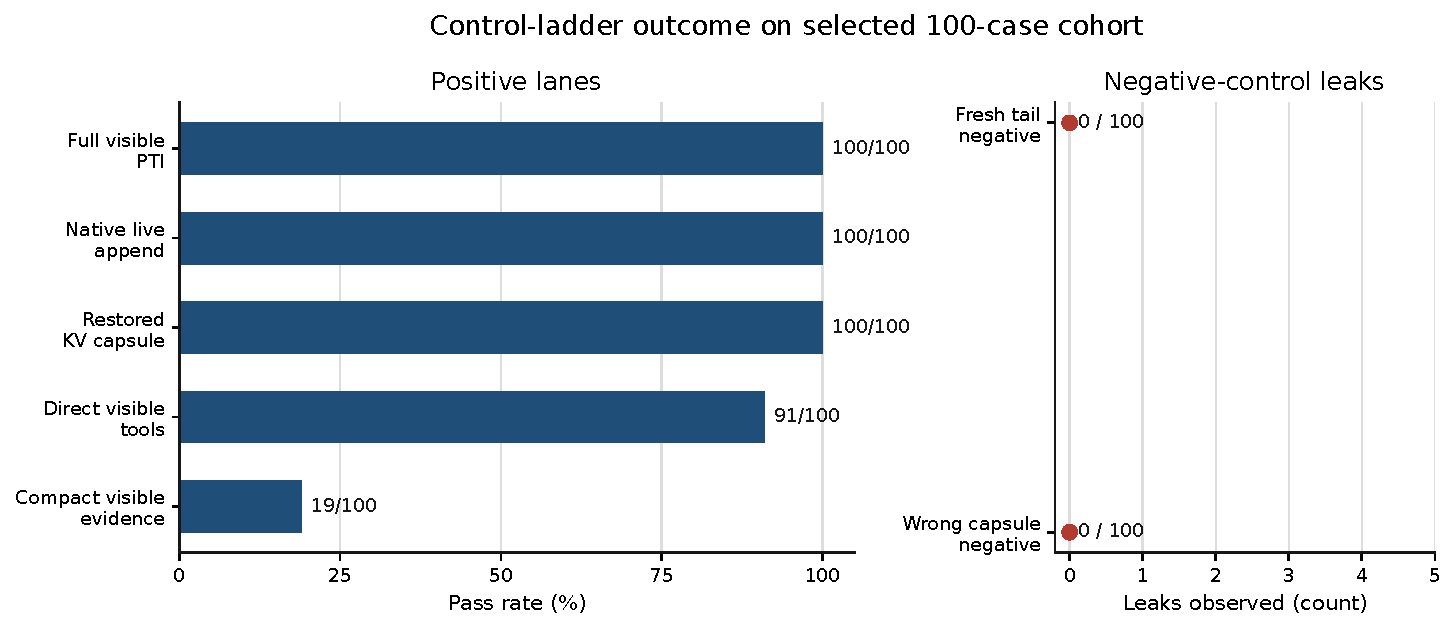
\includegraphics[width=\linewidth]{figures/figure-01-control-ladder.pdf}
  \caption{Control-ladder outcome on the selected 100-case cohort. Positive lanes are shown as pass rate; negative controls are shown separately as leak count. Restored KV matches both full-visible and native-live controls on all selected cases, while fresh-tail and wrong-capsule controls produce zero leaks.}
  \label{fig:control-ladder}
\end{figure}

\subsection{Constrained Structured Tool Interface}

PTI is the name used in this runtime for a constrained structured local tool interface. It gives the model a compact contract for emitting tool/function-call plans after capsule restore, without replaying the full stable tool/interface schema as fresh visible text. This design is motivated by function-calling benchmarks that expose tool selection, argument construction, and multi-call composition as distinct reliability problems \cite{bfcl2025,qin2023toollm,patil2023gorilla}. PTI is narrower than arbitrary programmatic tool calling: it is a controlled execution surface built for deterministic local-agent evaluation.

\subsection{Control Ladder}

The selected-cohort mechanism run uses seven controls: full visible PTI, native live append, restored KV capsule, fresh-tail negative, wrong-capsule negative, direct visible tools, and compact visible evidence. Native live append reads the same stable prefix and task tail without save/restore. Restored KV restores the saved hidden state and appends the same task tail. Fresh-tail and wrong-capsule lanes test whether the answer leaks from the tail alone or from irrelevant hidden state. Direct visible tools and compact visible evidence are visible-text ablations.

\section{Results}

\subsection{Restored KV Preserves Native Prefix Behavior}

Restored KV Capsule matched both full visible PTI and native live append at 100/100. The harness also recorded 100/100 native/restored output-hash parity: for every selected case, the restored-capsule lane produced the same hashed output as the native live-append comparator. This supports the claim that restored hidden state preserved the useful stable-prefix behavior for these cases. It should not be read as a claim about bit-identical internal KV tensors. Table~\ref{tab:mechanism} summarizes the positive mechanism lanes.

\begin{table}[h]
\centering
\begin{tabular}{lllll}
\toprule
Lane & Role & Pass & Mean ms & Median ms \\
\midrule
Full visible PTI & Positive reference & 100/100 & 6,766.7 & 6,252.9 \\
Native live append & Live prefix+tail comparator & 100/100 & 6,782.7 & 6,253.5 \\
Restored KV Capsule & Saved prefix-state restore & 100/100 & 8,513.8 & 8,042.3 \\
\bottomrule
\end{tabular}
\caption{Selected-cohort positive mechanism lanes. This result supports semantic preservation, not a low-level restore speed claim.}
\label{tab:mechanism}
\end{table}

\subsection{Negative Controls Stay Closed}

Both negative controls stayed closed with zero leaks. The fresh-tail lane shows that task tails alone did not contain enough visible information to solve the selected cases. The wrong-capsule lane shows that irrelevant hidden state did not substitute for the correct stable prefix. These controls support prefix dependence on this cohort; they do not establish general safety of arbitrary capsule reuse.

\subsection{PTI Helps Relative to Direct Visible Tools}

Full visible PTI passed 100/100, while direct visible tools passed 91/100. This does not establish universal PTI superiority, but it shows that interface shape affected reliability on the selected cohort, consistent with prior tool-use evaluations where API representation and call construction are central failure modes \cite{bfcl2025,qin2023toollm,patil2023gorilla}.

\subsection{Compact Visible Evidence Does Not Explain the Result}

Compact visible evidence passed 19/100, far below restored KV Capsule at 100/100. A compact visible representation did not reproduce the behavior obtained from restored hidden state. This result distinguishes the capsule mechanism from text-memory and reflection-style approaches that preserve continuity by writing information back into the prompt.

\subsection{Repeated-Work Runtime Comparison}

On the repeated-work stream, KV Capsule + PTI had the best pass rate, smallest new visible input burden after restore, and lowest cumulative wall time among the reported system lanes. The small KV input number does not mean the model had only 3,900 tokens of useful context. The stable prefix was already represented by restored hidden KV state; the reported visible count is only the fresh task-tail/control text appended after each restore. The text-threaded baseline compacted the conversation during the run; its token field is cumulative reported visible-input telemetry from the local-agent route. The comparison is a practical local-agent runtime result: same local model family, different runtime contracts, and a local-inference setting where repeated prefill and transcript growth are material systems costs.

\begin{table}[h]
\centering
\resizebox{\linewidth}{!}{%
\begin{tabular}{llllll}
\toprule
System & Pass & Stable context & Wall ms & Visible input & Compactions \\
\midrule
KV Capsule + PTI & 100/100 & Restored hidden state & 853,499 & 3,900 & 0 \\
Text-threaded baseline & 86/100 & Natural compaction & 11,813,816 & 245,774,883 & 89 \\
Text-threaded, no observed compaction & 87/100 & Text thread & 11,521,048 & 243,088,507 & 0 \\
\bottomrule
\end{tabular}
}
\caption{Repeated-work systems comparison. This is a practical runtime comparison, not a prompt-identical KV-versus-compaction mechanism comparison. Visible-input fields are route-reported cumulative telemetry, not clean per-task token accounting.}
\label{tab:repeated-work}
\end{table}

\begin{figure}[t]
  \centering
  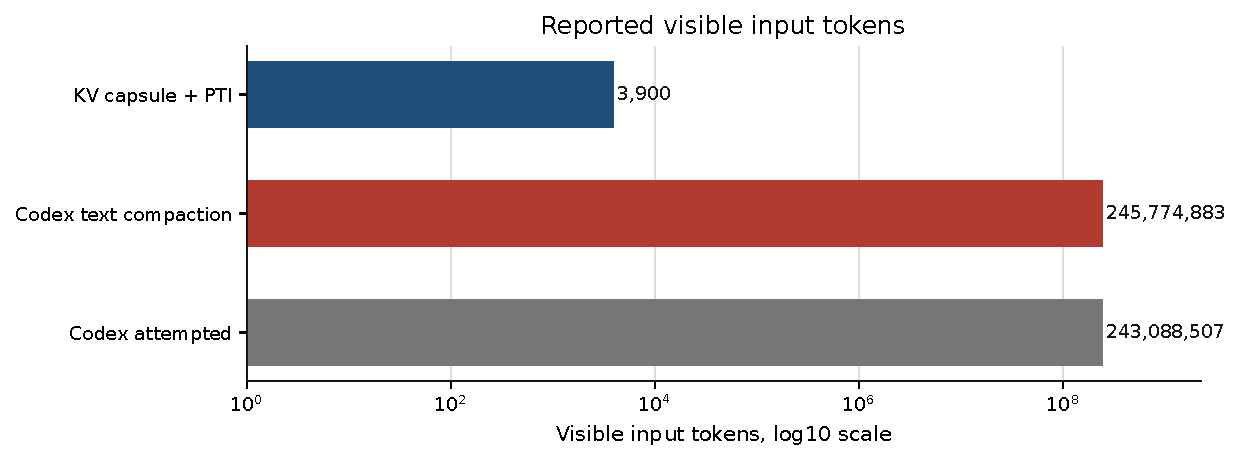
\includegraphics[width=\linewidth]{figures/figure-04-visible-input-tokens.pdf}
  \caption{Repeated-work visible input burden. Log scale is used because the runtime gap is several orders of magnitude. The baseline telemetry is cumulative reported burden, not clean per-task token accounting.}
  \label{fig:visible-input}
\end{figure}

\begin{figure}[t]
  \centering
  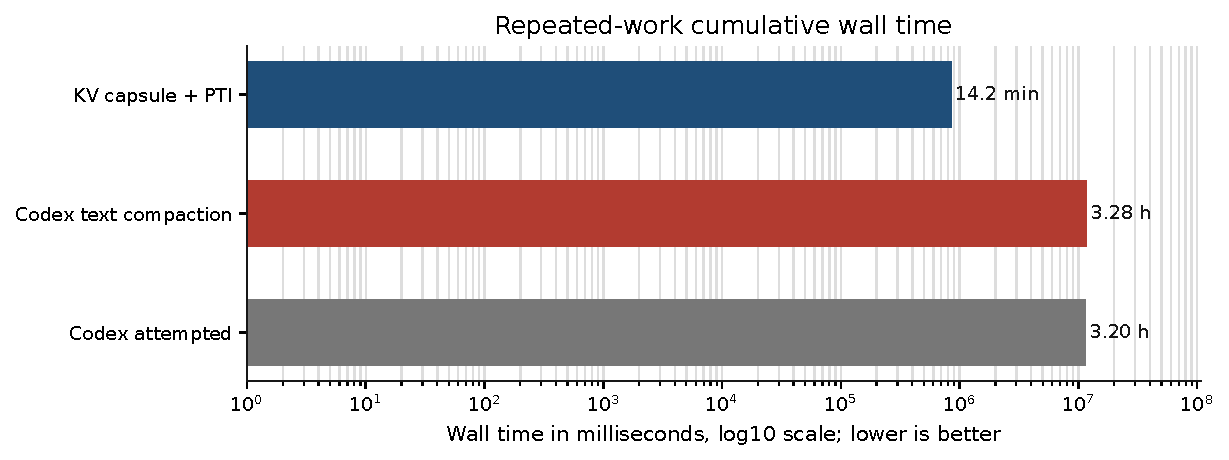
\includegraphics[width=\linewidth]{figures/figure-05-wall-time.pdf}
  \caption{Repeated-work cumulative wall time. KV completed the stream in 14.2 minutes versus 3.28 hours for the natural text-compaction lane.}
  \label{fig:wall-time}
\end{figure}

\section{Discussion}

\subsection{Why Attention Preservation Matters}

The selected-cohort result is primarily a mechanism result, not a general benchmark result. Restored KV matched native live append while the fresh-tail and wrong-capsule controls stayed closed. That pattern supports the mechanism claim: the successful tail response depended on the stable prefix state, and the saved capsule preserved that state well enough for the tested tasks. Unlike PagedAttention or RadixAttention, which optimize serving and shared-prefix execution \cite{kwon2023pagedattention,zheng2023sglang}, this experiment asks whether restored KV state preserves task behavior in a local tool-use harness.

This is a different primitive from text compaction. A summary may preserve useful facts, but it is not the model's computed state after reading the original prefix. KV Capsules expose a local-runtime option that is not normally available to users of hosted chat products: treat the model's computed prefix state as reusable execution state. That differs from memory architectures that rehydrate context as text, such as MemGPT and Reflexion \cite{packer2023memgpt,shinn2023reflexion}.

\subsection{Where the Speed Claim Lives}

The mechanism run does not show restored KV is intrinsically faster; restored KV was slower than full visible and native live append on mean total latency. The speed result appears in repeated work. When stable context would otherwise be carried through many turns, KV Capsule + PTI reduced the repeated visible contract to small task tails and avoided repeated natural-language compaction.

\subsection{How to Read the Baseline}

The text-threaded baseline is a practical local-agent route, not a prompt-identical scientific control. It is included because real agent systems have overhead: tool surfaces, summaries, logs, validation, and retries. The comparison is therefore narrow: under the tested local repeated-work route, KV Capsule + PTI compared favorably to the tested natural text-compaction route.

\section{Limitations}

The evaluation is scoped to local Gemma 4 12B experiments. The selected cohort is quality-gated and BFCL-derived; it is not an official BFCL leaderboard submission, and the selected-cohort pass rates should not be read as distribution-wide BFCL performance.

The text-threaded baseline is a practical runtime comparison, not a prompt-identical mechanism comparison. It uses the same model family but a different runtime contract. Baseline visible-input telemetry is cumulative route-reported burden, not clean per-task token accounting.

The selected-cohort mechanism run supports semantic preservation, not low-level restore speed. In that run, restored KV was slower than native live append on mean latency. The speed result appears only in repeated work, where stable context can be amortized across tasks.

Fresh-tail and wrong-capsule controls test leakage and prefix dependence only on this selected cohort. They do not establish general safety of hidden-state reuse, arbitrary capsule interchange, or out-of-distribution tool behavior.

The 89 compaction events are supported by tracked summary artifacts, but the raw Windows session JSONL is not present in this checkout. The compaction baseline is therefore diagnostic for practical repeated-work overhead, not a causal analysis of which individual summaries helped or hurt.

PTI is a structured local tool interface for agent runtimes, not arbitrary programmatic tool calling. The results should be read as evidence about this controlled harness and workload, not as a claim about all tool-use interfaces.

\appendix
\section{BFCL Non-Live Calibration}

The initial full non-live evaluator check scored 69.88\% on BFCL's leaderboard-style Non-Live AST Acc calculation. That score is an unweighted average over the non-live AST groups: simple, multiple, parallel, and parallel-multiple. The scoreable generated-record count across all seven local non-live files was 969/1390, or 69.71\%, with irrelevance reported separately at 57.08\%. This result is useful as an end-to-end calibration of the export and evaluator path. It is not used as the final official benchmark number for this draft, and it is not a public leaderboard submission.

\begin{figure}[h]
  \centering
  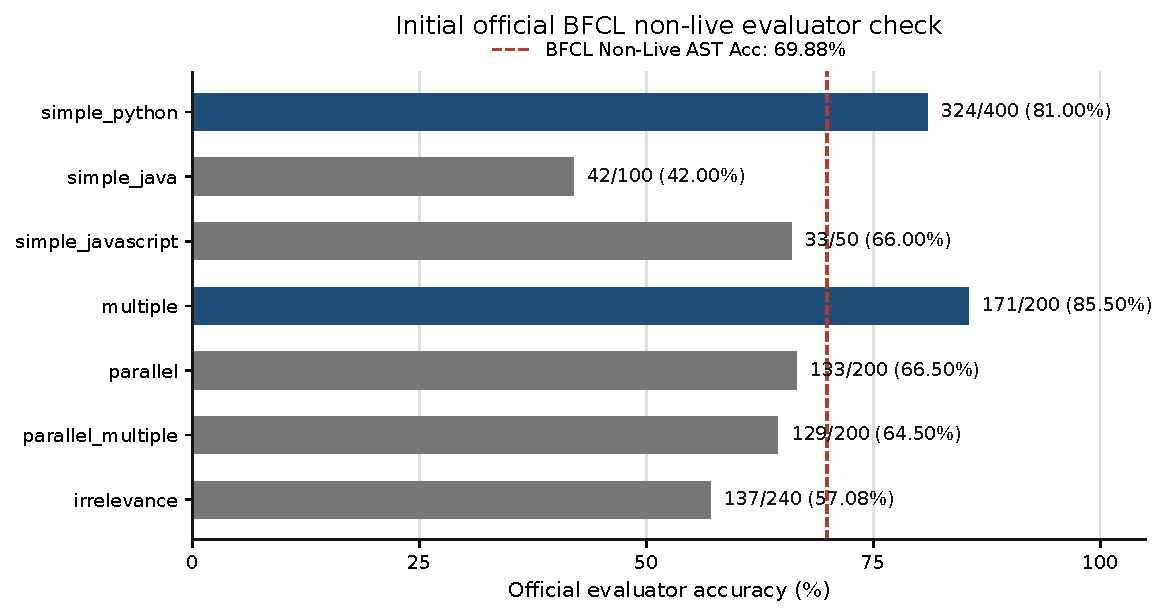
\includegraphics[width=\linewidth]{figures/figure-07-initial-official-bfcl.pdf}
  \caption{Initial full BFCL non-live official-evaluator check. Category accuracies are shown for the first exported prediction run; the dashed line marks BFCL Non-Live AST Acc.}
  \label{fig:bfcl-initial}
\end{figure}

\begin{figure}[h]
  \centering
  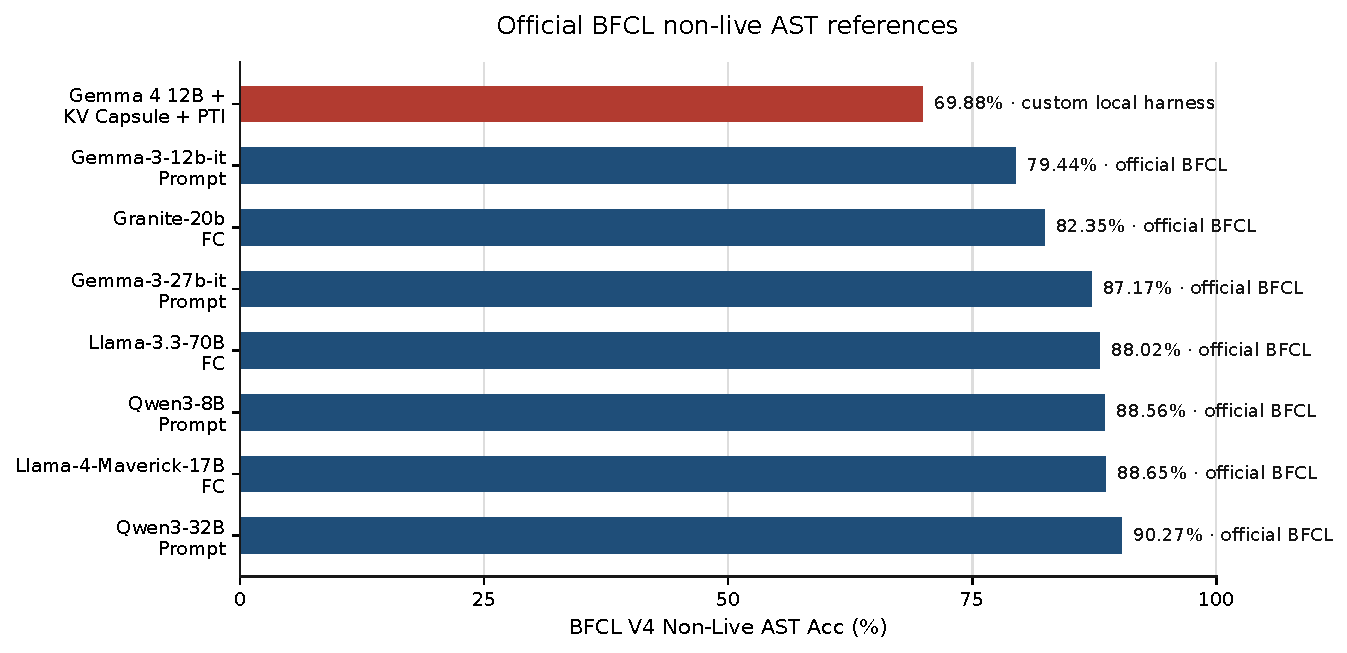
\includegraphics[width=\linewidth]{figures/figure-08-bfcl-reference-comparison.pdf}
  \caption{BFCL V4 Non-Live AST reference comparison. This is a non-live-only comparison against public BFCL rows. It should not be read as overall leaderboard rank, hosted-model cost comparison, or evidence about live/multi-turn BFCL categories.}
  \label{fig:bfcl-reference}
\end{figure}

\section{Artifacts and Data Availability}

All paper-facing artifacts, analysis scripts, figure manifests, and arXiv sources are available in the public repository:
\begin{center}
\url{https://github.com/fraction12/ai-research-lab}
\end{center}
The arXiv v1 source snapshot is tagged as \texttt{arxiv-v1.0}:
\begin{center}
\url{https://github.com/fraction12/ai-research-lab/tree/arxiv-v1.0}
\end{center}

The reproducibility map is:
\begin{itemize}[leftmargin=*]
  \item The selected-cohort mechanism directory contains the summary table and findings memo for the control ladder.
  \item The repeated-work comparison artifacts contain the speed summary and failure analysis used for the practical systems comparison.
  \item The BFCL calibration directory contains the official-evaluator summary, context-burden summary, and latency derivation.
  \item The paper-artifacts directory contains the figure manifest and scripts used to regenerate the plots.
  \item The arXiv directory contains the exact LaTeX source, bibliography, compiled figures, and compiled PDF.
\end{itemize}

These files live under the paper track, \texttt{research/02-quality-gated-stateful-kv-reuse/}. Exact filenames and relative paths are listed in the repository README and artifact manifests.

\bibliographystyle{plain}
\bibliography{references}

\end{document}
